% Options for packages loaded elsewhere
\PassOptionsToPackage{unicode}{hyperref}
\PassOptionsToPackage{hyphens}{url}
%
\documentclass[
]{article}
\usepackage{amsmath,amssymb}
\usepackage{iftex}
\ifPDFTeX
  \usepackage[T1]{fontenc}
  \usepackage[utf8]{inputenc}
  \usepackage{textcomp} % provide euro and other symbols
\else % if luatex or xetex
  \usepackage{unicode-math} % this also loads fontspec
  \defaultfontfeatures{Scale=MatchLowercase}
  \defaultfontfeatures[\rmfamily]{Ligatures=TeX,Scale=1}
\fi
\usepackage{lmodern}
\ifPDFTeX\else
  % xetex/luatex font selection
\fi
% Use upquote if available, for straight quotes in verbatim environments
\IfFileExists{upquote.sty}{\usepackage{upquote}}{}
\IfFileExists{microtype.sty}{% use microtype if available
  \usepackage[]{microtype}
  \UseMicrotypeSet[protrusion]{basicmath} % disable protrusion for tt fonts
}{}
\makeatletter
\@ifundefined{KOMAClassName}{% if non-KOMA class
  \IfFileExists{parskip.sty}{%
    \usepackage{parskip}
  }{% else
    \setlength{\parindent}{0pt}
    \setlength{\parskip}{6pt plus 2pt minus 1pt}}
}{% if KOMA class
  \KOMAoptions{parskip=half}}
\makeatother
\usepackage{xcolor}
\usepackage[margin=1in]{geometry}
\usepackage{longtable,booktabs,array}
\usepackage{calc} % for calculating minipage widths
% Correct order of tables after \paragraph or \subparagraph
\usepackage{etoolbox}
\makeatletter
\patchcmd\longtable{\par}{\if@noskipsec\mbox{}\fi\par}{}{}
\makeatother
% Allow footnotes in longtable head/foot
\IfFileExists{footnotehyper.sty}{\usepackage{footnotehyper}}{\usepackage{footnote}}
\makesavenoteenv{longtable}
\usepackage{graphicx}
\makeatletter
\def\maxwidth{\ifdim\Gin@nat@width>\linewidth\linewidth\else\Gin@nat@width\fi}
\def\maxheight{\ifdim\Gin@nat@height>\textheight\textheight\else\Gin@nat@height\fi}
\makeatother
% Scale images if necessary, so that they will not overflow the page
% margins by default, and it is still possible to overwrite the defaults
% using explicit options in \includegraphics[width, height, ...]{}
\setkeys{Gin}{width=\maxwidth,height=\maxheight,keepaspectratio}
% Set default figure placement to htbp
\makeatletter
\def\fps@figure{htbp}
\makeatother
\setlength{\emergencystretch}{3em} % prevent overfull lines
\providecommand{\tightlist}{%
  \setlength{\itemsep}{0pt}\setlength{\parskip}{0pt}}
\setcounter{secnumdepth}{-\maxdimen} % remove section numbering
\usepackage{float} \floatplacement{figure}{H}
\ifLuaTeX
  \usepackage{selnolig}  % disable illegal ligatures
\fi
\IfFileExists{bookmark.sty}{\usepackage{bookmark}}{\usepackage{hyperref}}
\IfFileExists{xurl.sty}{\usepackage{xurl}}{} % add URL line breaks if available
\urlstyle{same}
\hypersetup{
  pdftitle={Report for policy makers},
  pdfauthor={Becky Yuen},
  hidelinks,
  pdfcreator={LaTeX via pandoc}}

\title{Report for policy makers}
\author{Becky Yuen}
\date{}

\begin{document}
\maketitle

\hypertarget{introduction}{%
\subsection{Introduction}\label{introduction}}

This is the overall report for the analysis on the
\href{https://search.gesis.org/research_data/ZA7500}{European Value
Study (EVS) from 2017} which is a survey research program on how
Europeans think about family, work, religion, politics, and society. We
are mainly interested in Europeans thoughts on two questions:

\begin{enumerate}
\def\labelenumi{\arabic{enumi}.}
\tightlist
\item
  When a mother works for pay, do Europeans think the children suffer?
\item
  When jobs are scarce, do Europeans think employers should give
  priority to local people over immigrants?
\end{enumerate}

\hypertarget{descriptives-of-variables}{%
\subsection{Descriptives of variables}\label{descriptives-of-variables}}

In the following table, the variables are:

\begin{enumerate}
\def\labelenumi{\arabic{enumi}.}
\tightlist
\item
  \texttt{v72} represents the first question of interest (1-strongly
  agree, 2-agree, 3-disagree, or 4-strongly disagree)
\item
  \texttt{v80} represents the second question of interest (1-strongly
  agree, 2-agree, 3-neither agree nor disagree, 4-disagree, or
  5-strongly disagree)
\item
  \texttt{sex} (1-male or 2-female)
\item
  \texttt{age} (years)
\item
  \texttt{education} (1-lower, 2-medium, or 3-higher)
\end{enumerate}

\begin{longtable}[]{@{}
  >{\centering\arraybackslash}p{(\columnwidth - 4\tabcolsep) * \real{0.2222}}
  >{\centering\arraybackslash}p{(\columnwidth - 4\tabcolsep) * \real{0.2222}}
  >{\centering\arraybackslash}p{(\columnwidth - 4\tabcolsep) * \real{0.2222}}@{}}
\caption{Descriptive table for continuous variables}\tabularnewline
\toprule\noalign{}
\begin{minipage}[b]{\linewidth}\centering
v72
\end{minipage} & \begin{minipage}[b]{\linewidth}\centering
v80
\end{minipage} & \begin{minipage}[b]{\linewidth}\centering
age
\end{minipage} \\
\midrule\noalign{}
\endfirsthead
\toprule\noalign{}
\begin{minipage}[b]{\linewidth}\centering
v72
\end{minipage} & \begin{minipage}[b]{\linewidth}\centering
v80
\end{minipage} & \begin{minipage}[b]{\linewidth}\centering
age
\end{minipage} \\
\midrule\noalign{}
\endhead
\bottomrule\noalign{}
\endlastfoot
Min. :1.000 & Min. :1.000 & Min. :18.00 \\
1st Qu.:2.000 & 1st Qu.:1.000 & 1st Qu.:35.00 \\
Median :3.000 & Median :2.000 & Median :50.00 \\
Mean :2.713 & Mean :2.313 & Mean :49.57 \\
3rd Qu.:3.000 & 3rd Qu.:3.000 & 3rd Qu.:64.00 \\
Max. :4.000 & Max. :5.000 & Max. :82.00 \\
\end{longtable}

\begin{longtable}[]{@{}lrr@{}}
\caption{Descriptive table for categorical variables}\tabularnewline
\toprule\noalign{}
Education & Sex & Freq \\
\midrule\noalign{}
\endfirsthead
\toprule\noalign{}
Education & Sex & Freq \\
\midrule\noalign{}
\endhead
\bottomrule\noalign{}
\endlastfoot
Lower & M & 4727.00 \\
Medium & M & 11992.00 \\
Higher & M & 8351.00 \\
Lower & F & 6802.00 \\
Medium & F & 13835.00 \\
Higher & F & 11048.00 \\
\end{longtable}

\hypertarget{graphs}{%
\subsection{Graphs}\label{graphs}}

\begin{figure}

{\centering 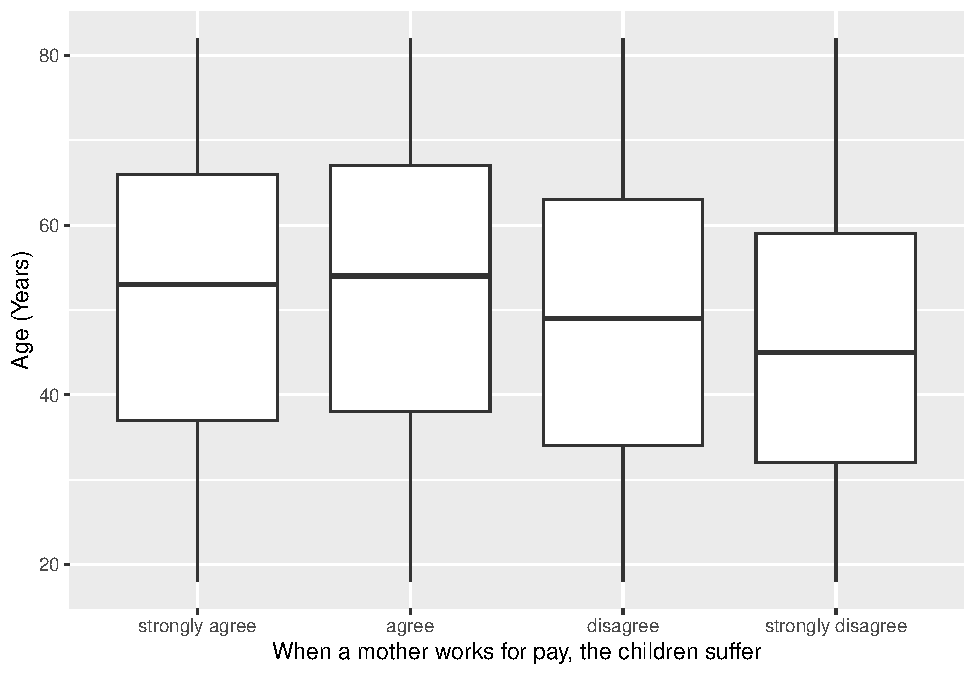
\includegraphics[width=0.65\linewidth]{Report-for-policy-makers_files/figure-latex/plot_v72-1} 

}

\caption{Boxplot for first question of interest (v72)}\label{fig:plot_v72}
\end{figure}

We can see that the distributions of age among categories of opinion are
quite similar.\\

\begin{figure}

{\centering 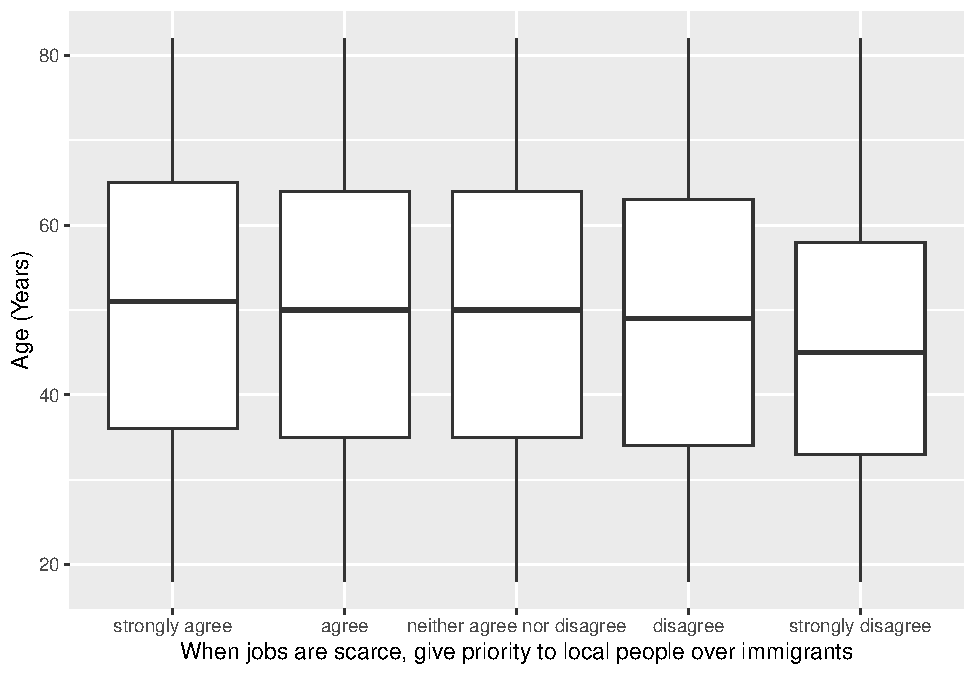
\includegraphics[width=0.65\linewidth]{Report-for-policy-makers_files/figure-latex/plot_v80-1} 

}

\caption{Boxplot for second question of interest (v80)}\label{fig:plot_v80}
\end{figure}

Same as the previous plot, we can see that the distributions of age
among categories of opinion are quite similar.

\hypertarget{regression-analysis}{%
\subsection{Regression Analysis}\label{regression-analysis}}

\hypertarget{model-v72-age-sqrttextage-sex-education}{%
\subsubsection{\texorpdfstring{Model: v72 \textasciitilde{} age +
\(\sqrt{\text{age}}\) + sex +
education}{Model: v72 \textasciitilde{} age + \textbackslash sqrt\{\textbackslash text\{age\}\} + sex + education}}\label{model-v72-age-sqrttextage-sex-education}}

\begin{longtable}[]{@{}
  >{\centering\arraybackslash}p{(\columnwidth - 8\tabcolsep) * \real{0.3194}}
  >{\centering\arraybackslash}p{(\columnwidth - 8\tabcolsep) * \real{0.1667}}
  >{\centering\arraybackslash}p{(\columnwidth - 8\tabcolsep) * \real{0.1806}}
  >{\centering\arraybackslash}p{(\columnwidth - 8\tabcolsep) * \real{0.1528}}
  >{\centering\arraybackslash}p{(\columnwidth - 8\tabcolsep) * \real{0.1806}}@{}}
\toprule\noalign{}
\begin{minipage}[b]{\linewidth}\centering
~
\end{minipage} & \begin{minipage}[b]{\linewidth}\centering
Estimate
\end{minipage} & \begin{minipage}[b]{\linewidth}\centering
Std. Error
\end{minipage} & \begin{minipage}[b]{\linewidth}\centering
t value
\end{minipage} & \begin{minipage}[b]{\linewidth}\centering
Pr(\textgreater\textbar t\textbar)
\end{minipage} \\
\midrule\noalign{}
\endhead
\bottomrule\noalign{}
\endlastfoot
\textbf{(Intercept)} & 2.728 & 0.09723 & 28.06 & 4.655e-172 \\
\textbf{age} & -0.004774 & 0.002203 & -2.167 & 0.03023 \\
\textbf{sqrt(age)} & -0.001149 & 0.02976 & -0.03861 & 0.9692 \\
\textbf{sex-female} & 0.06448 & 0.007257 & 8.886 & 6.537e-19 \\
\textbf{education-medium} & 0.1233 & 0.009852 & 12.51 & 7.325e-36 \\
\textbf{education-higher} & 0.4012 & 0.01046 & 38.36 & 7.574e-318 \\
\end{longtable}

\begin{longtable}[]{@{}
  >{\centering\arraybackslash}p{(\columnwidth - 6\tabcolsep) * \real{0.2083}}
  >{\centering\arraybackslash}p{(\columnwidth - 6\tabcolsep) * \real{0.3056}}
  >{\centering\arraybackslash}p{(\columnwidth - 6\tabcolsep) * \real{0.1389}}
  >{\centering\arraybackslash}p{(\columnwidth - 6\tabcolsep) * \real{0.2361}}@{}}
\caption{Fitting linear model: v72 \textasciitilde{} age + sqrt(age) +
sex + education}\tabularnewline
\toprule\noalign{}
\begin{minipage}[b]{\linewidth}\centering
Observations
\end{minipage} & \begin{minipage}[b]{\linewidth}\centering
Residual Std. Error
\end{minipage} & \begin{minipage}[b]{\linewidth}\centering
\(R^2\)
\end{minipage} & \begin{minipage}[b]{\linewidth}\centering
Adjusted \(R^2\)
\end{minipage} \\
\midrule\noalign{}
\endfirsthead
\toprule\noalign{}
\begin{minipage}[b]{\linewidth}\centering
Observations
\end{minipage} & \begin{minipage}[b]{\linewidth}\centering
Residual Std. Error
\end{minipage} & \begin{minipage}[b]{\linewidth}\centering
\(R^2\)
\end{minipage} & \begin{minipage}[b]{\linewidth}\centering
Adjusted \(R^2\)
\end{minipage} \\
\midrule\noalign{}
\endhead
\bottomrule\noalign{}
\endlastfoot
56755 & 0.8576 & 0.04769 & 0.04761 \\
\end{longtable}

The coefficient estimate for \texttt{sex} is 0.0644834 which means that
the effect of a female respondent compared to a male is positive. The
corresponding \(p\)-value is \ensuremath{6.5368574\times 10^{-19}} which
is smaller than 0.05. Thus, \texttt{sex} is significant in the model.

\hypertarget{model-v80-age-sqrttextage-sex-education}{%
\subsubsection{\texorpdfstring{Model: v80 \textasciitilde{} age +
\(\sqrt{\text{age}}\) + sex +
education}{Model: v80 \textasciitilde{} age + \textbackslash sqrt\{\textbackslash text\{age\}\} + sex + education}}\label{model-v80-age-sqrttextage-sex-education}}

\begin{longtable}[]{@{}
  >{\centering\arraybackslash}p{(\columnwidth - 8\tabcolsep) * \real{0.3194}}
  >{\centering\arraybackslash}p{(\columnwidth - 8\tabcolsep) * \real{0.1667}}
  >{\centering\arraybackslash}p{(\columnwidth - 8\tabcolsep) * \real{0.1806}}
  >{\centering\arraybackslash}p{(\columnwidth - 8\tabcolsep) * \real{0.1389}}
  >{\centering\arraybackslash}p{(\columnwidth - 8\tabcolsep) * \real{0.1806}}@{}}
\toprule\noalign{}
\begin{minipage}[b]{\linewidth}\centering
~
\end{minipage} & \begin{minipage}[b]{\linewidth}\centering
Estimate
\end{minipage} & \begin{minipage}[b]{\linewidth}\centering
Std. Error
\end{minipage} & \begin{minipage}[b]{\linewidth}\centering
t value
\end{minipage} & \begin{minipage}[b]{\linewidth}\centering
Pr(\textgreater\textbar t\textbar)
\end{minipage} \\
\midrule\noalign{}
\endhead
\bottomrule\noalign{}
\endlastfoot
\textbf{(Intercept)} & 2.344 & 0.1427 & 16.43 & 1.646e-60 \\
\textbf{age} & -0.003823 & 0.003232 & -1.183 & 0.2369 \\
\textbf{sqrt(age)} & 0.006788 & 0.04367 & 0.1554 & 0.8765 \\
\textbf{sex-female} & -0.03151 & 0.01065 & -2.959 & 0.003084 \\
\textbf{education-medium} & -0.03504 & 0.01446 & -2.424 & 0.01536 \\
\textbf{education-higher} & 0.4238 & 0.01535 & 27.61 & 9.812e-167 \\
\end{longtable}

\begin{longtable}[]{@{}
  >{\centering\arraybackslash}p{(\columnwidth - 6\tabcolsep) * \real{0.2083}}
  >{\centering\arraybackslash}p{(\columnwidth - 6\tabcolsep) * \real{0.3056}}
  >{\centering\arraybackslash}p{(\columnwidth - 6\tabcolsep) * \real{0.1389}}
  >{\centering\arraybackslash}p{(\columnwidth - 6\tabcolsep) * \real{0.2361}}@{}}
\caption{Fitting linear model: v80 \textasciitilde{} age + sqrt(age) +
sex + education}\tabularnewline
\toprule\noalign{}
\begin{minipage}[b]{\linewidth}\centering
Observations
\end{minipage} & \begin{minipage}[b]{\linewidth}\centering
Residual Std. Error
\end{minipage} & \begin{minipage}[b]{\linewidth}\centering
\(R^2\)
\end{minipage} & \begin{minipage}[b]{\linewidth}\centering
Adjusted \(R^2\)
\end{minipage} \\
\midrule\noalign{}
\endfirsthead
\toprule\noalign{}
\begin{minipage}[b]{\linewidth}\centering
Observations
\end{minipage} & \begin{minipage}[b]{\linewidth}\centering
Residual Std. Error
\end{minipage} & \begin{minipage}[b]{\linewidth}\centering
\(R^2\)
\end{minipage} & \begin{minipage}[b]{\linewidth}\centering
Adjusted \(R^2\)
\end{minipage} \\
\midrule\noalign{}
\endhead
\bottomrule\noalign{}
\endlastfoot
56755 & 1.258 & 0.03124 & 0.03115 \\
\end{longtable}

The coefficient estimate for \texttt{sex} is -0.0315131 which means that
the effect of a female respondent compared to a male is negative. The
corresponding \(p\)-value is 0.003084 which is smaller than 0.05. Thus,
\texttt{sex} is significant in the model.

\end{document}
